% ============================================================================
% CHAPTER 1G: AEROSPACE SYSTEMS
% ============================================================================

\section{Aerospace Systems}
\label{sec:aerospace}

Aerospace systems present unique control challenges: operation in three dimensions, coupling between axes, varying dynamics with flight conditions, and stringent safety requirements.

% ============================================================================
\subsection{Aircraft Longitudinal Dynamics}
\label{subsec:longitudinal}
% ============================================================================

\begin{figure}[htbp]
\centering
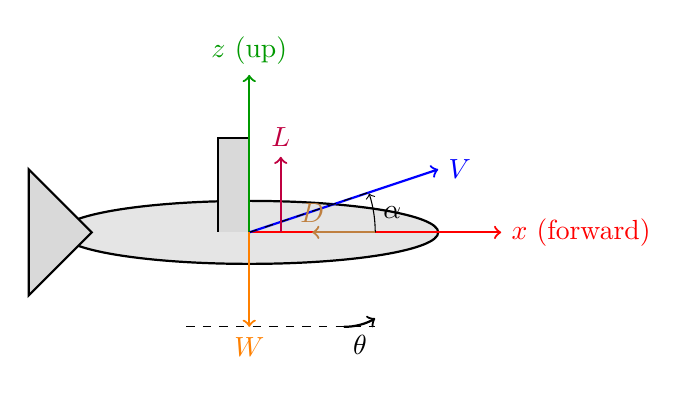
\begin{tikzpicture}[scale=0.8]
    % Aircraft body
    \draw[thick, fill=gray!20] (0,0) ellipse (3 and 0.5);
    \draw[thick, fill=gray!30] (-2.5,0) -- (-3.5,1) -- (-3.5,-1) -- cycle;
    \draw[thick, fill=gray!30] (0,0) -- (0,1.5) -- (-0.5,1.5) -- (-0.5,0);

    % Axes
    \draw[->, thick, red] (0,0) -- (4,0) node[right] {$x$ (forward)};
    \draw[->, thick, green!60!black] (0,0) -- (0,2.5) node[above] {$z$ (up)};

    % Velocity vector
    \draw[->, thick, blue] (0,0) -- (3,1) node[right] {$V$};

    % Angles
    \draw[->] (2,0) arc (0:18:2) node[midway, right] {$\alpha$};
    \draw[dashed] (0,0) -- (2,0.67);

    % Pitch angle
    \draw[->, thick] (1.5,-1.5) arc (-90:-60:1) node[midway, below] {$\theta$};
    \draw[dashed] (-1,-1.5) -- (2,-1.5);

    % Forces
    \draw[->, thick, orange] (0,0) -- (0,-1.5) node[below] {$W$};
    \draw[->, thick, purple] (0.5,0) -- (0.5,1.2) node[above] {$L$};
    \draw[->, thick, brown] (2,0) -- (1,0) node[above] {$D$};
\end{tikzpicture}
\caption{Aircraft longitudinal plane showing forces and angles.}
\label{fig:aircraft_longitudinal}
\end{figure}

\subsubsection{State Variables}

\begin{itemize}
    \item $u$ = forward velocity perturbation (m/s)
    \item $w$ = vertical velocity perturbation (m/s)
    \item $q$ = pitch rate (rad/s)
    \item $\theta$ = pitch angle (rad)
\end{itemize}

\subsubsection{Linearized Equations of Motion}

\begin{equation}
\begin{bmatrix} \dot{u} \\ \dot{w} \\ \dot{q} \\ \dot{\theta} \end{bmatrix} =
\begin{bmatrix}
X_u & X_w & 0 & -g \\
Z_u & Z_w & U_0 & 0 \\
M_u & M_w & M_q & 0 \\
0 & 0 & 1 & 0
\end{bmatrix}
\begin{bmatrix} u \\ w \\ q \\ \theta \end{bmatrix} +
\begin{bmatrix} X_{\delta_e} \\ Z_{\delta_e} \\ M_{\delta_e} \\ 0 \end{bmatrix} \delta_e
\end{equation}

where $\delta_e$ is elevator deflection and $X_u$, $Z_w$, etc. are stability derivatives.

\subsubsection{Characteristic Modes}

The longitudinal dynamics typically have two modes:

\textbf{Short Period Mode:}
\begin{itemize}
    \item Fast oscillation (1-3 seconds period)
    \item Primarily $\alpha$ and $q$ motion
    \item Well-damped ($\zeta \approx 0.3-0.7$)
\end{itemize}

Approximate transfer function:
\begin{equation}
\frac{\alpha(s)}{\delta_e(s)} \approx \frac{Z_{\delta_e}/U_0}{s^2 - (M_q + M_{\dot{\alpha}} + Z_w/U_0)s + (Z_w M_q/U_0 - M_w)}
\end{equation}

\textbf{Phugoid Mode:}
\begin{itemize}
    \item Slow oscillation (30-100 seconds period)
    \item Exchange between kinetic and potential energy
    \item Lightly damped ($\zeta \approx 0.04-0.1$)
\end{itemize}

Approximate frequency and damping:
\begin{align}
\omega_p &\approx \sqrt{2}\frac{g}{U_0} \\
\zeta_p &\approx \frac{1}{\sqrt{2}}\frac{C_D}{C_L}
\end{align}

\begin{examplebox}[title=Example 1.14: Boeing 747 Longitudinal Modes]
At cruise ($U_0 = 250$ m/s, altitude 10 km):

Short period:
\begin{itemize}
    \item $\omega_{sp} = 0.9$ rad/s, $\zeta_{sp} = 0.35$
    \item Period: $T_{sp} = 2\pi/\omega_{sp} = 7$ s
\end{itemize}

Phugoid:
\begin{itemize}
    \item $\omega_p = 0.06$ rad/s, $\zeta_p = 0.05$
    \item Period: $T_p = 2\pi/\omega_p = 105$ s
\end{itemize}
\end{examplebox}

% ============================================================================
\subsection{Aircraft Body Axes and Rotational Dynamics}
\label{subsec:body_axes}
% ============================================================================

\begin{figure}[htbp]
\centering
\begin{tikzpicture}[scale=1.2]
    % Aircraft body (fuselage)
    \draw[thick, fill=UofSCGarnet!30] (0,0) ellipse (2.5 and 0.4);

    % Wing
    \draw[thick, fill=UofSCAtlantic!20] (-1.5,-0.2) -- (-2.8,-0.8) -- (-2.8,-1.2) -- (-1.5,-0.6) -- cycle;
    \draw[thick, fill=UofSCAtlantic!20] (-1.5,-0.2) -- (-2.8,0.8) -- (-2.8,1.2) -- (-1.5,0.6) -- cycle;

    % Vertical stabilizer (tail)
    \draw[thick, fill=UofSCCongaree!20] (2.2,-0.3) -- (2.7,-0.3) -- (2.7,-1.2) -- (2.2,-0.3);

    % Body-fixed coordinate axes
    \draw[->, thick, UofSCGarnet] (0,0) -- (3,0) node[right] {$x$ (pitch)};
    \draw[->, thick, UofSCGarnet] (0,0) -- (0,2) node[above] {$z$ (roll)};
    \draw[->, thick, UofSCGarnet] (0,0) -- (-1.5,-1.5) node[below left] {$y$ (yaw)};

    % Pitch moment (nose up)
    \draw[->, thick, UofSCHorseshoe] (3.5,0.5) arc (0:60:0.8) node[midway, right] {$M$ (pitch)};

    % Roll moment (right wing down)
    \draw[->, thick, UofSCHorseshoe] (0.5,1.8) arc (90:30:0.7) node[midway, above] {$L$ (roll)};

    % Yaw moment (nose right)
    \draw[->, thick, UofSCHorseshoe] (-1.5,-1.8) arc (-45:45:0.8) node[midway, below] {$N$ (yaw)};

    % Angular velocities
    \node[text=UofSCAtlantic] at (0,3.2) {Angular rates: $p$ (roll), $q$ (pitch), $r$ (yaw)};
\end{tikzpicture}
\caption{Aircraft body-fixed coordinate axes showing pitch, roll, and yaw moments with associated angular velocities.}
\label{fig:aircraft_body_axes}
\end{figure}

% ============================================================================
\subsection{Aircraft Lateral-Directional Dynamics}
\label{subsec:lateral}
% ============================================================================

\subsubsection{State Variables}

\begin{itemize}
    \item $\beta$ = sideslip angle (rad)
    \item $p$ = roll rate (rad/s)
    \item $r$ = yaw rate (rad/s)
    \item $\phi$ = bank angle (rad)
\end{itemize}

\subsubsection{Characteristic Modes}

\textbf{Dutch Roll:}
\begin{itemize}
    \item Coupled yaw-roll oscillation
    \item Period: 3-10 seconds
    \item Damping varies with aircraft design
\end{itemize}

\textbf{Roll Mode:}
\begin{itemize}
    \item Pure rolling motion
    \item First-order, typically fast (time constant 0.5-2 s)
\end{itemize}

\textbf{Spiral Mode:}
\begin{itemize}
    \item Slow divergence or convergence
    \item Often slightly unstable (acceptable if slow)
\end{itemize}

% ============================================================================
\subsection{Rocket Dynamics}
\label{subsec:rocket}
% ============================================================================

\begin{figure}[htbp]
\centering
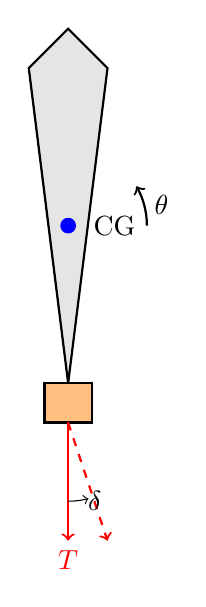
\begin{tikzpicture}
    % Rocket body
    \draw[thick, fill=gray!20] (0,0) -- (0.5,4) -- (0,4.5) -- (-0.5,4) -- (0,0);
    \draw[thick, fill=orange!50] (-0.3,0) -- (0.3,0) -- (0.3,-0.5) -- (-0.3,-0.5) -- cycle;

    % Thrust vector
    \draw[->, thick, red] (0,-0.5) -- (0,-2) node[below] {$T$};

    % Gimbal angle
    \draw[->, thick, red, dashed] (0,-0.5) -- (0.5,-2);
    \draw[->] (0,-1.5) arc (-90:-75:1) node[midway, right] {$\delta$};

    % Center of mass
    \fill[blue] (0,2) circle (0.1);
    \node[right] at (0.2,2) {CG};

    % Attitude
    \draw[->, thick] (1,2) arc (0:30:1) node[midway, right] {$\theta$};
\end{tikzpicture}
\caption{Rocket with thrust vector control.}
\label{fig:rocket}
\end{figure}

\subsubsection{Pitch Dynamics (Simplified)}

For a rocket with thrust vector control:
\begin{equation}
I_{yy}\ddot{\theta} = T \cdot \ell_T \cdot \delta
\end{equation}

where:
\begin{itemize}
    \item $I_{yy}$ = pitch moment of inertia
    \item $T$ = thrust
    \item $\ell_T$ = distance from CG to gimbal point
    \item $\delta$ = gimbal angle
\end{itemize}

Transfer function:
\begin{equation}
\frac{\Theta(s)}{\delta(s)} = \frac{T\ell_T/I_{yy}}{s^2} = \frac{K_r}{s^2}
\end{equation}

This is a double integrator---marginally stable and requires feedback for control.

\subsubsection{Aerodynamic Effects}

With aerodynamic forces, additional terms appear:
\begin{equation}
I_{yy}\ddot{\theta} = T\ell_T\delta + M_\alpha\alpha + M_q q
\end{equation}

For a statically unstable rocket ($M_\alpha > 0$), the system has a pole in the right half-plane.

% ============================================================================
\subsection{Satellite Attitude Dynamics}
\label{subsec:satellite}
% ============================================================================

\begin{figure}[htbp]
\centering
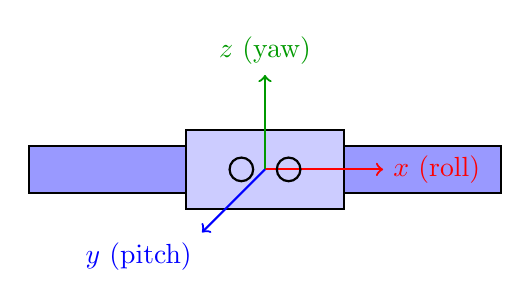
\begin{tikzpicture}
    % Satellite body
    \draw[thick, fill=blue!20] (-1,-0.5) rectangle (1,0.5);

    % Solar panels
    \draw[thick, fill=blue!40] (-3,-0.3) rectangle (-1,0.3);
    \draw[thick, fill=blue!40] (1,-0.3) rectangle (3,0.3);

    % Body axes
    \draw[->, thick, red] (0,0) -- (1.5,0) node[right] {$x$ (roll)};
    \draw[->, thick, green!60!black] (0,0) -- (0,1.2) node[above] {$z$ (yaw)};
    \draw[->, thick, blue] (0,0) -- (-0.8,-0.8) node[below left] {$y$ (pitch)};

    % Reaction wheels (symbolic)
    \draw[thick] (0.3,0) circle (0.15);
    \draw[thick] (-0.3,0) circle (0.15);
\end{tikzpicture}
\caption{Satellite with body-fixed axes.}
\label{fig:satellite}
\end{figure}

\subsubsection{Euler's Equations}

\begin{align}
I_{xx}\dot{\omega}_x + (I_{zz} - I_{yy})\omega_y\omega_z &= \tau_x \\
I_{yy}\dot{\omega}_y + (I_{xx} - I_{zz})\omega_z\omega_x &= \tau_y \\
I_{zz}\dot{\omega}_z + (I_{yy} - I_{xx})\omega_x\omega_y &= \tau_z
\end{align}

\subsubsection{Linearized Single-Axis Model}

For small angles about one axis:
\begin{equation}
I\ddot{\theta} = \tau
\end{equation}

Transfer function:
\begin{equation}
\frac{\Theta(s)}{\tau(s)} = \frac{1}{Is^2}
\end{equation}

\subsubsection{Reaction Wheel Dynamics}

A reaction wheel applies torque by changing its angular momentum:
\begin{equation}
\tau_{\text{satellite}} = -I_w\dot{\omega}_w
\end{equation}

Combined system:
\begin{equation}
I_s\ddot{\theta} = -I_w\dot{\omega}_w = I_w\ddot{\theta}_w
\end{equation}

% ============================================================================
\subsection{Quadrotor Dynamics}
\label{subsec:quadrotor}
% ============================================================================

\begin{figure}[htbp]
\centering
\begin{tikzpicture}[scale=1.1]
    % Central body
    \draw[thick, fill=UofSCGarnet!30] (-0.4,-0.25) rectangle (0.4,0.25);

    % Cross arms (orthogonal)
    \draw[thick, UofSCGarnet] (-2.5,0) -- (2.5,0);
    \draw[thick, UofSCGarnet] (0,-2.5) -- (0,2.5);

    % Motor/propeller circles
    \draw[thick, fill=UofSCAtlantic!20] (2,0) circle (0.4);
    \draw[thick, fill=UofSCAtlantic!20] (-2,0) circle (0.4);
    \draw[thick, fill=UofSCAtlantic!20] (0,2) circle (0.4);
    \draw[thick, fill=UofSCAtlantic!20] (0,-2) circle (0.4);

    % Propeller orientation indicators
    \draw[thick, UofSCAtlantic] (2.2,-0.2) -- (1.8,0.2);
    \draw[thick, UofSCAtlantic] (-2.2,-0.2) -- (-1.8,0.2);
    \draw[thick, UofSCAtlantic] (-0.2,2.2) -- (0.2,1.8);
    \draw[thick, UofSCAtlantic] (-0.2,-2.2) -- (0.2,-1.8);

    % Thrust forces (upward)
    \draw[->, thick, UofSCHorseshoe] (2,0.5) -- (2,1.8) node[above, font=\small] {$F_1$};
    \draw[->, thick, UofSCHorseshoe] (-2,0.5) -- (-2,1.8) node[above, font=\small] {$F_2$};
    \draw[->, thick, UofSCHorseshoe] (0,2.5) -- (0,3.8) node[above, font=\small] {$F_3$};
    \draw[->, thick, UofSCHorseshoe] (0,-2.5) -- (0,-3.8) node[below, font=\small] {$F_4$};

    % Angular velocities labels
    \draw[->, thick, UofSCCongaree] (0.5,0) arc (0:90:0.6) node[midway, above right, font=\small] {$\dot{\psi}$ (yaw)};
    \draw[->, thick, UofSCCongaree] (2.5,-0.3) arc (0:60:0.5) node[midway, right, font=\small] {$\dot{\phi}$ (roll)};
    \draw[->, thick, UofSCCongaree] (-0.3,2.5) arc (0:-60:0.5) node[midway, left, font=\small] {$\dot{\theta}$ (pitch)};

    % Body frame axes
    \draw[->, thick, UofSCGarnet] (0,0) -- (1.2,0) node[right, font=\small] {$x$};
    \draw[->, thick, UofSCGarnet] (0,0) -- (0,1.2) node[above, font=\small] {$z$};
\end{tikzpicture}
\caption{Quadrotor free body diagram showing thrust forces at each rotor and angular velocities for roll, pitch, and yaw control.}
\label{fig:quadrotor_fbd}
\end{figure}

\begin{figure}[htbp]
\centering
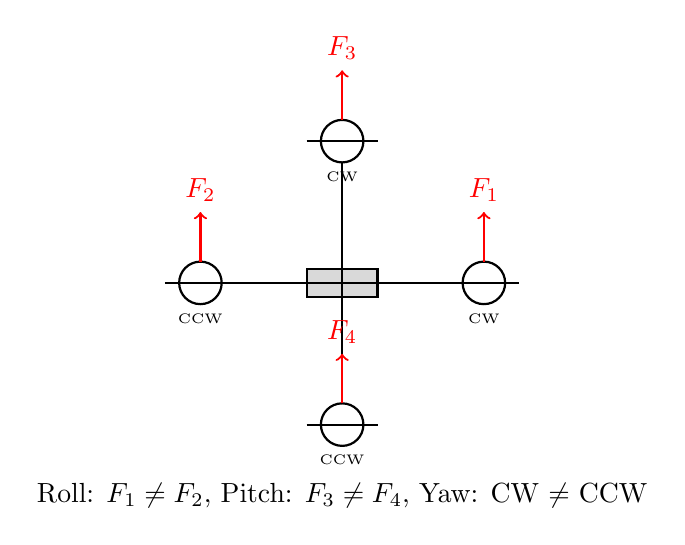
\begin{tikzpicture}[scale=0.9]
    % Body
    \draw[thick, fill=gray!30] (-0.5,-0.2) rectangle (0.5,0.2);

    % Arms
    \draw[thick] (-2,0) -- (2,0);
    \draw[thick] (0,-2) -- (0,2);

    % Motors/propellers
    \foreach \x/\y/\rot in {2/0/CW, -2/0/CCW, 0/2/CW, 0/-2/CCW} {
        \draw[thick, fill=white] (\x,\y) circle (0.3);
        \draw[thick] (\x-0.5,\y) -- (\x+0.5,\y);
        \node[font=\tiny] at (\x,\y-0.5) {\rot};
    }

    % Thrust arrows
    \draw[->, thick, red] (2,0.3) -- (2,1) node[above] {$F_1$};
    \draw[->, thick, red] (-2,0.3) -- (-2,1) node[above] {$F_2$};
    \draw[->, thick, red] (0,2.3) -- (0,3) node[above] {$F_3$};
    \draw[->, thick, red] (0,-1.7) -- (0,-1) node[above] {$F_4$};

    % Labels
    \node at (0,-3) {Roll: $F_1 \neq F_2$, Pitch: $F_3 \neq F_4$, Yaw: CW $\neq$ CCW};
\end{tikzpicture}
\caption{Quadrotor configuration showing rotor positions and control mixing.}
\label{fig:quadrotor}
\end{figure}

\subsubsection{Control Inputs}

\begin{align}
\text{Total thrust:} \quad T &= F_1 + F_2 + F_3 + F_4 \\
\text{Roll torque:} \quad \tau_\phi &= \ell(F_1 - F_2) \\
\text{Pitch torque:} \quad \tau_\theta &= \ell(F_3 - F_4) \\
\text{Yaw torque:} \quad \tau_\psi &= k_\tau(F_1 + F_2 - F_3 - F_4)
\end{align}

\subsubsection{Equations of Motion}

Translational (in body frame):
\begin{align}
m\ddot{x} &= -mg\sin\theta \\
m\ddot{y} &= mg\cos\theta\sin\phi \\
m\ddot{z} &= mg\cos\theta\cos\phi - T
\end{align}

Rotational:
\begin{align}
I_{xx}\ddot{\phi} &= \tau_\phi \\
I_{yy}\ddot{\theta} &= \tau_\theta \\
I_{zz}\ddot{\psi} &= \tau_\psi
\end{align}

\subsubsection{Linearized Model (Hover)}

Near hover ($\phi, \theta, \psi \approx 0$):
\begin{equation}
\ddot{\phi} = \frac{\ell}{I_{xx}}(F_1 - F_2), \quad
\ddot{\theta} = \frac{\ell}{I_{yy}}(F_3 - F_4), \quad
\ddot{z} = g - \frac{T}{m}
\end{equation}

% ============================================================================
\subsection{Spacecraft Orbital Mechanics}
\label{subsec:orbital}
% ============================================================================

\subsubsection{Hill-Clohessy-Wiltshire Equations}

Relative motion near a circular reference orbit:
\begin{align}
\ddot{x} - 2n\dot{y} - 3n^2 x &= a_x \\
\ddot{y} + 2n\dot{x} &= a_y \\
\ddot{z} + n^2 z &= a_z
\end{align}

where $n = \sqrt{\mu/a^3}$ is the orbital rate.

The out-of-plane motion ($z$) is decoupled and is a simple harmonic oscillator.

The in-plane motion ($x$, $y$) is coupled, with the solution:
\begin{equation}
x(t) = (4 - 3\cos nt)x_0 + \frac{\sin nt}{n}\dot{x}_0 + \frac{2(1-\cos nt)}{n}\dot{y}_0
\end{equation}

% ============================================================================
\subsection{Exercises: Aerospace Systems}
% ============================================================================

\begin{exercise}
An aircraft has short-period approximation:
\begin{equation}
\frac{\alpha(s)}{\delta_e(s)} = \frac{-2}{s^2 + 1.5s + 4}
\end{equation}
\begin{enumerate}[label=(\alph*)]
    \item Find the natural frequency and damping ratio
    \item Is this response acceptable for a fighter aircraft?
    \item Sketch the step response
\end{enumerate}
\end{exercise}

\begin{exercise}
A rocket has pitch moment of inertia $I_{yy} = 10^6$ kg$\cdot$m$^2$, thrust $T = 10^6$ N, and gimbal arm $\ell_T = 20$ m.
\begin{enumerate}[label=(\alph*)]
    \item Find the transfer function from gimbal angle to pitch rate
    \item Design a proportional controller to achieve 1 rad/s$^2$ pitch acceleration per degree of gimbal
\end{enumerate}
\end{exercise}

\begin{exercise}
A satellite reaction wheel has inertia $I_w = 0.01$ kg$\cdot$m$^2$ and the satellite has inertia $I_s = 100$ kg$\cdot$m$^2$ about one axis.
\begin{enumerate}[label=(\alph*)]
    \item If the wheel accelerates at 100 rad/s$^2$, find the satellite angular acceleration
    \item Find the maximum satellite rate if the wheel is limited to 6000 rpm
\end{enumerate}
\end{exercise}

\begin{exercise}
A quadrotor has mass 1.5 kg, arm length 0.25 m, and moment of inertia $I_{xx} = I_{yy} = 0.02$ kg$\cdot$m$^2$.
\begin{enumerate}[label=(\alph*)]
    \item Find the hover thrust per motor
    \item Derive the transfer function from motor force differential to roll angle
    \item If motor response is modeled as first-order with $\tau = 0.05$ s, find the complete roll transfer function
\end{enumerate}
\end{exercise}

\begin{exercise}
A satellite has inertia $I = 50$ kg$\cdot$m$^2$ about the pitch axis. Two reaction wheels are available with inertias $I_w = 0.5$ kg$\cdot$m$^2$ each, located 90\degree apart about the body axes.
\begin{enumerate}[label=(\alph*)]
    \item Write the coupled equations for pitch-yaw control using both wheels
    \item If the pitch wheel accelerates at 200 rad/s$^2$, find the satellite pitch angular acceleration
    \item Design a control law to achieve zero final angular rate when the pitch wheel reaches 3000 rpm
\end{enumerate}
\end{exercise}

\begin{exercise}
An aircraft has longitudinal dynamics with short-period natural frequency $\omega_n = 1.2$ rad/s and damping $\zeta = 0.45$. The phugoid has $\omega_p = 0.08$ rad/s and $\zeta_p = 0.06$.
\begin{enumerate}[label=(\alph*)]
    \item Sketch the pole-zero map for the longitudinal system
    \item Calculate the time constants for each mode
    \item What type of controller (P, PI, or PD) would be best for elevator control? Why?
\end{enumerate}
\end{exercise}

\begin{exercise}
A rocket undergoes pitch control with gimbal actuation. The rocket parameters are: $I_{yy} = 2 \times 10^6$ kg$\cdot$m$^2$, thrust $T = 5 \times 10^6$ N, gimbal arm $\ell = 10$ m, and aerodynamic damping coefficient $M_q = -3 \times 10^5$ N$\cdot$m$\cdot$s/rad.
\begin{enumerate}[label=(\alph*)]
    \item Derive the transfer function from gimbal angle $\delta$ to pitch rate $q$
    \item Find the system poles and determine stability
    \item Design a proportional controller to limit pitch rate to 5 deg/s for 1\degree gimbal command
\end{enumerate}
\end{exercise}

\begin{exercise}
A quadrotor must perform a roll maneuver from level flight. It has mass $m = 2$ kg, arm length $\ell = 0.3$ m, and $I_{xx} = 0.025$ kg$\cdot$m$^2$.
\begin{enumerate}[label=(\alph*)]
    \item For a rolling maneuver command of 0.5 rad/s$^2$, calculate the required roll torque
    \item Find the force differential between motors: $\Delta F = F_1 - F_2$
    \item If available motor thrust is 10 N each, what is the maximum roll acceleration?
\end{enumerate}
\end{exercise}

\begin{exercise}
Consider a satellite attitude control system using a three-axis reaction wheel assembly. The satellite inertia matrix is diagonal: $I_{xx} = 80$, $I_{yy} = 100$, $I_{zz} = 120$ kg$\cdot$m$^2$.
\begin{enumerate}[label=(\alph*)]
    \item Write the decoupled single-axis control law for each axis: $\tau = I \ddot{\theta}$
    \item If maximum wheel torque is 0.2 N$\cdot$m, find the maximum angular acceleration for each axis
    \item Design a PD controller for the yaw axis: $\tau = K_p e + K_d \dot{e}$, with desired natural frequency 0.1 rad/s and damping ratio 0.7
\end{enumerate}
\end{exercise}
